% Created by tikzDevice version 0.12.6 on 2025-04-17 10:36:56
% !TEX encoding = UTF-8 Unicode
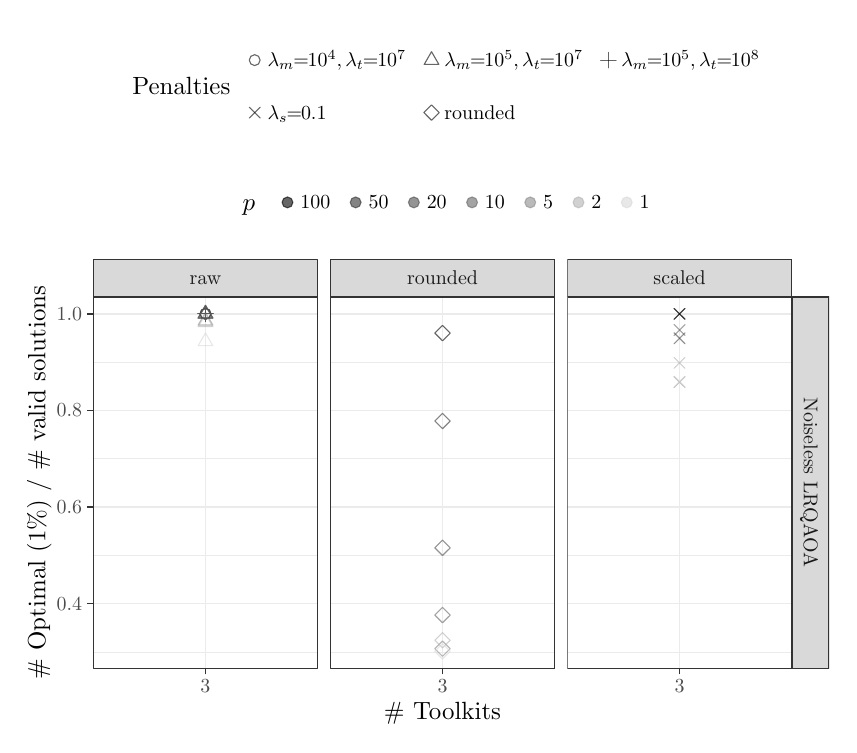
\begin{tikzpicture}[x=1pt,y=1pt]
\definecolor{fillColor}{RGB}{255,255,255}
\path[use as bounding box,fill=fillColor,fill opacity=0.00] (0,0) rectangle (289.58,251.81);
\begin{scope}
\path[clip] (  0.00,  0.00) rectangle (289.58,251.81);
\definecolor{drawColor}{RGB}{255,255,255}
\definecolor{fillColor}{RGB}{255,255,255}

\path[draw=drawColor,line width= 0.5pt,line join=round,line cap=round,fill=fillColor] (  0.00,  0.00) rectangle (289.58,251.81);
\end{scope}
\begin{scope}
\path[clip] ( 23.68, 20.35) rectangle (104.83,154.50);
\definecolor{fillColor}{RGB}{255,255,255}

\path[fill=fillColor] ( 23.68, 20.35) rectangle (104.83,154.50);
\definecolor{drawColor}{gray}{0.92}

\path[draw=drawColor,line width= 0.2pt,line join=round] ( 23.68, 26.26) --
	(104.83, 26.26);

\path[draw=drawColor,line width= 0.2pt,line join=round] ( 23.68, 61.16) --
	(104.83, 61.16);

\path[draw=drawColor,line width= 0.2pt,line join=round] ( 23.68, 96.05) --
	(104.83, 96.05);

\path[draw=drawColor,line width= 0.2pt,line join=round] ( 23.68,130.95) --
	(104.83,130.95);

\path[draw=drawColor,line width= 0.5pt,line join=round] ( 23.68, 43.71) --
	(104.83, 43.71);

\path[draw=drawColor,line width= 0.5pt,line join=round] ( 23.68, 78.61) --
	(104.83, 78.61);

\path[draw=drawColor,line width= 0.5pt,line join=round] ( 23.68,113.50) --
	(104.83,113.50);

\path[draw=drawColor,line width= 0.5pt,line join=round] ( 23.68,148.40) --
	(104.83,148.40);

\path[draw=drawColor,line width= 0.5pt,line join=round] ( 64.25, 20.35) --
	( 64.25,154.50);
\definecolor{drawColor}{RGB}{140,140,140}

\path[draw=drawColor,draw opacity=0.60,line width= 0.4pt,line join=round,line cap=round] ( 64.25,148.96) --
	( 66.89,144.38) --
	( 61.61,144.38) --
	cycle;
\definecolor{drawColor}{RGB}{77,77,77}

\path[draw=drawColor,draw opacity=0.60,line width= 0.4pt,line join=round,line cap=round] ( 64.25,151.45) --
	( 66.89,146.88) --
	( 61.61,146.88) --
	cycle;
\definecolor{drawColor}{RGB}{0,0,0}

\path[draw=drawColor,draw opacity=0.60,line width= 0.4pt,line join=round,line cap=round] ( 61.48,148.40) -- ( 67.03,148.40);

\path[draw=drawColor,draw opacity=0.60,line width= 0.4pt,line join=round,line cap=round] ( 64.25,145.63) -- ( 64.25,151.18);

\path[draw=drawColor,draw opacity=0.60,line width= 0.4pt,line join=round,line cap=round] ( 64.25,148.40) circle (  1.96);
\definecolor{drawColor}{RGB}{51,51,51}

\path[draw=drawColor,draw opacity=0.60,line width= 0.4pt,line join=round,line cap=round] ( 64.25,148.40) circle (  1.96);
\definecolor{drawColor}{RGB}{77,77,77}

\path[draw=drawColor,draw opacity=0.60,line width= 0.4pt,line join=round,line cap=round] ( 64.25,148.40) circle (  1.96);
\definecolor{drawColor}{RGB}{179,179,179}

\path[draw=drawColor,draw opacity=0.60,line width= 0.4pt,line join=round,line cap=round] ( 64.25,148.39) --
	( 66.89,143.81) --
	( 61.61,143.81) --
	cycle;
\definecolor{drawColor}{RGB}{51,51,51}

\path[draw=drawColor,draw opacity=0.60,line width= 0.4pt,line join=round,line cap=round] ( 64.25,151.45) --
	( 66.89,146.88) --
	( 61.61,146.88) --
	cycle;
\definecolor{drawColor}{RGB}{217,217,217}

\path[draw=drawColor,draw opacity=0.60,line width= 0.4pt,line join=round,line cap=round] ( 64.25,141.48) --
	( 66.89,136.90) --
	( 61.61,136.90) --
	cycle;
\definecolor{drawColor}{RGB}{51,51,51}

\path[draw=drawColor,draw opacity=0.60,line width= 0.4pt,line join=round,line cap=round] ( 61.48,148.40) -- ( 67.03,148.40);

\path[draw=drawColor,draw opacity=0.60,line width= 0.4pt,line join=round,line cap=round] ( 64.25,145.63) -- ( 64.25,151.18);
\definecolor{drawColor}{RGB}{102,102,102}

\path[draw=drawColor,draw opacity=0.60,line width= 0.4pt,line join=round,line cap=round] ( 61.48,148.40) -- ( 67.03,148.40);

\path[draw=drawColor,draw opacity=0.60,line width= 0.4pt,line join=round,line cap=round] ( 64.25,145.63) -- ( 64.25,151.18);

\path[draw=drawColor,draw opacity=0.60,line width= 0.4pt,line join=round,line cap=round] ( 64.25,151.45) --
	( 66.89,146.88) --
	( 61.61,146.88) --
	cycle;
\definecolor{drawColor}{gray}{0.20}

\path[draw=drawColor,line width= 0.5pt,line join=round,line cap=round] ( 23.68, 20.35) rectangle (104.83,154.50);
\end{scope}
\begin{scope}
\path[clip] (109.33, 20.35) rectangle (190.48,154.50);
\definecolor{fillColor}{RGB}{255,255,255}

\path[fill=fillColor] (109.33, 20.35) rectangle (190.48,154.50);
\definecolor{drawColor}{gray}{0.92}

\path[draw=drawColor,line width= 0.2pt,line join=round] (109.33, 26.26) --
	(190.48, 26.26);

\path[draw=drawColor,line width= 0.2pt,line join=round] (109.33, 61.16) --
	(190.48, 61.16);

\path[draw=drawColor,line width= 0.2pt,line join=round] (109.33, 96.05) --
	(190.48, 96.05);

\path[draw=drawColor,line width= 0.2pt,line join=round] (109.33,130.95) --
	(190.48,130.95);

\path[draw=drawColor,line width= 0.5pt,line join=round] (109.33, 43.71) --
	(190.48, 43.71);

\path[draw=drawColor,line width= 0.5pt,line join=round] (109.33, 78.61) --
	(190.48, 78.61);

\path[draw=drawColor,line width= 0.5pt,line join=round] (109.33,113.50) --
	(190.48,113.50);

\path[draw=drawColor,line width= 0.5pt,line join=round] (109.33,148.40) --
	(190.48,148.40);

\path[draw=drawColor,line width= 0.5pt,line join=round] (149.90, 20.35) --
	(149.90,154.50);
\definecolor{drawColor}{RGB}{0,0,0}

\path[draw=drawColor,draw opacity=0.60,line width= 0.4pt,line join=round,line cap=round] (147.13,141.44) --
	(149.90,144.21) --
	(152.68,141.44) --
	(149.90,138.66) --
	cycle;
\definecolor{drawColor}{RGB}{140,140,140}

\path[draw=drawColor,draw opacity=0.60,line width= 0.4pt,line join=round,line cap=round] (147.13, 27.41) --
	(149.90, 30.19) --
	(152.68, 27.41) --
	(149.90, 24.64) --
	cycle;
\definecolor{drawColor}{RGB}{102,102,102}

\path[draw=drawColor,draw opacity=0.60,line width= 0.4pt,line join=round,line cap=round] (147.13, 39.55) --
	(149.90, 42.33) --
	(152.68, 39.55) --
	(149.90, 36.78) --
	cycle;
\definecolor{drawColor}{RGB}{77,77,77}

\path[draw=drawColor,draw opacity=0.60,line width= 0.4pt,line join=round,line cap=round] (147.13, 63.85) --
	(149.90, 66.63) --
	(152.68, 63.85) --
	(149.90, 61.08) --
	cycle;
\definecolor{drawColor}{RGB}{179,179,179}

\path[draw=drawColor,draw opacity=0.60,line width= 0.4pt,line join=round,line cap=round] (147.13, 30.45) --
	(149.90, 33.23) --
	(152.68, 30.45) --
	(149.90, 27.68) --
	cycle;
\definecolor{drawColor}{RGB}{217,217,217}

\path[draw=drawColor,draw opacity=0.60,line width= 0.4pt,line join=round,line cap=round] (147.13, 26.45) --
	(149.90, 29.23) --
	(152.68, 26.45) --
	(149.90, 23.68) --
	cycle;
\definecolor{drawColor}{RGB}{51,51,51}

\path[draw=drawColor,draw opacity=0.60,line width= 0.4pt,line join=round,line cap=round] (147.13,109.67) --
	(149.90,112.44) --
	(152.68,109.67) --
	(149.90,106.89) --
	cycle;
\definecolor{drawColor}{gray}{0.20}

\path[draw=drawColor,line width= 0.5pt,line join=round,line cap=round] (109.33, 20.35) rectangle (190.48,154.50);
\end{scope}
\begin{scope}
\path[clip] (194.98, 20.35) rectangle (276.13,154.50);
\definecolor{fillColor}{RGB}{255,255,255}

\path[fill=fillColor] (194.98, 20.35) rectangle (276.13,154.50);
\definecolor{drawColor}{gray}{0.92}

\path[draw=drawColor,line width= 0.2pt,line join=round] (194.98, 26.26) --
	(276.13, 26.26);

\path[draw=drawColor,line width= 0.2pt,line join=round] (194.98, 61.16) --
	(276.13, 61.16);

\path[draw=drawColor,line width= 0.2pt,line join=round] (194.98, 96.05) --
	(276.13, 96.05);

\path[draw=drawColor,line width= 0.2pt,line join=round] (194.98,130.95) --
	(276.13,130.95);

\path[draw=drawColor,line width= 0.5pt,line join=round] (194.98, 43.71) --
	(276.13, 43.71);

\path[draw=drawColor,line width= 0.5pt,line join=round] (194.98, 78.61) --
	(276.13, 78.61);

\path[draw=drawColor,line width= 0.5pt,line join=round] (194.98,113.50) --
	(276.13,113.50);

\path[draw=drawColor,line width= 0.5pt,line join=round] (194.98,148.40) --
	(276.13,148.40);

\path[draw=drawColor,line width= 0.5pt,line join=round] (235.56, 20.35) --
	(235.56,154.50);
\definecolor{drawColor}{RGB}{102,102,102}

\path[draw=drawColor,draw opacity=0.60,line width= 0.4pt,line join=round,line cap=round] (233.59,140.60) -- (237.52,144.52);

\path[draw=drawColor,draw opacity=0.60,line width= 0.4pt,line join=round,line cap=round] (233.59,144.52) -- (237.52,140.60);
\definecolor{drawColor}{RGB}{77,77,77}

\path[draw=drawColor,draw opacity=0.60,line width= 0.4pt,line join=round,line cap=round] (233.59,137.60) -- (237.52,141.53);

\path[draw=drawColor,draw opacity=0.60,line width= 0.4pt,line join=round,line cap=round] (233.59,141.53) -- (237.52,137.60);
\definecolor{drawColor}{RGB}{51,51,51}

\path[draw=drawColor,draw opacity=0.60,line width= 0.4pt,line join=round,line cap=round] (233.59,146.44) -- (237.52,150.36);

\path[draw=drawColor,draw opacity=0.60,line width= 0.4pt,line join=round,line cap=round] (233.59,150.36) -- (237.52,146.44);
\definecolor{drawColor}{RGB}{0,0,0}

\path[draw=drawColor,draw opacity=0.60,line width= 0.4pt,line join=round,line cap=round] (233.59,146.44) -- (237.52,150.36);

\path[draw=drawColor,draw opacity=0.60,line width= 0.4pt,line join=round,line cap=round] (233.59,150.36) -- (237.52,146.44);
\definecolor{drawColor}{RGB}{179,179,179}

\path[draw=drawColor,draw opacity=0.60,line width= 0.4pt,line join=round,line cap=round] (233.59,128.72) -- (237.52,132.65);

\path[draw=drawColor,draw opacity=0.60,line width= 0.4pt,line join=round,line cap=round] (233.59,132.65) -- (237.52,128.72);
\definecolor{drawColor}{RGB}{140,140,140}

\path[draw=drawColor,draw opacity=0.60,line width= 0.4pt,line join=round,line cap=round] (233.59,121.80) -- (237.52,125.72);

\path[draw=drawColor,draw opacity=0.60,line width= 0.4pt,line join=round,line cap=round] (233.59,125.72) -- (237.52,121.80);
\definecolor{drawColor}{RGB}{217,217,217}

\path[draw=drawColor,draw opacity=0.60,line width= 0.4pt,line join=round,line cap=round] (233.59,121.92) -- (237.52,125.84);

\path[draw=drawColor,draw opacity=0.60,line width= 0.4pt,line join=round,line cap=round] (233.59,125.84) -- (237.52,121.92);
\definecolor{drawColor}{gray}{0.20}

\path[draw=drawColor,line width= 0.5pt,line join=round,line cap=round] (194.98, 20.35) rectangle (276.13,154.50);
\end{scope}
\begin{scope}
\path[clip] ( 23.68,154.50) rectangle (104.83,167.94);
\definecolor{drawColor}{gray}{0.20}
\definecolor{fillColor}{gray}{0.85}

\path[draw=drawColor,line width= 0.5pt,line join=round,line cap=round,fill=fillColor] ( 23.68,154.50) rectangle (104.83,167.94);
\definecolor{drawColor}{gray}{0.10}

\node[text=drawColor,anchor=base,inner sep=0pt, outer sep=0pt, scale=  0.72] at ( 64.25,158.88) {raw};
\end{scope}
\begin{scope}
\path[clip] (109.33,154.50) rectangle (190.48,167.94);
\definecolor{drawColor}{gray}{0.20}
\definecolor{fillColor}{gray}{0.85}

\path[draw=drawColor,line width= 0.5pt,line join=round,line cap=round,fill=fillColor] (109.33,154.50) rectangle (190.48,167.94);
\definecolor{drawColor}{gray}{0.10}

\node[text=drawColor,anchor=base,inner sep=0pt, outer sep=0pt, scale=  0.72] at (149.90,158.88) {rounded};
\end{scope}
\begin{scope}
\path[clip] (194.98,154.50) rectangle (276.13,167.94);
\definecolor{drawColor}{gray}{0.20}
\definecolor{fillColor}{gray}{0.85}

\path[draw=drawColor,line width= 0.5pt,line join=round,line cap=round,fill=fillColor] (194.98,154.50) rectangle (276.13,167.94);
\definecolor{drawColor}{gray}{0.10}

\node[text=drawColor,anchor=base,inner sep=0pt, outer sep=0pt, scale=  0.72] at (235.56,158.88) {scaled};
\end{scope}
\begin{scope}
\path[clip] (276.13, 20.35) rectangle (289.58,154.50);
\definecolor{drawColor}{gray}{0.20}
\definecolor{fillColor}{gray}{0.85}

\path[draw=drawColor,line width= 0.5pt,line join=round,line cap=round,fill=fillColor] (276.13, 20.35) rectangle (289.58,154.50);
\definecolor{drawColor}{gray}{0.10}

\node[text=drawColor,rotate=-90.00,anchor=base,inner sep=0pt, outer sep=0pt, scale=  0.72] at (280.51, 87.43) {Noiseless LRQAOA};
\end{scope}
\begin{scope}
\path[clip] (  0.00,  0.00) rectangle (289.58,251.81);
\definecolor{drawColor}{gray}{0.20}

\path[draw=drawColor,line width= 0.5pt,line join=round] ( 64.25, 18.10) --
	( 64.25, 20.35);
\end{scope}
\begin{scope}
\path[clip] (  0.00,  0.00) rectangle (289.58,251.81);
\definecolor{drawColor}{gray}{0.30}

\node[text=drawColor,anchor=base,inner sep=0pt, outer sep=0pt, scale=  0.72] at ( 64.25, 11.62) {3};
\end{scope}
\begin{scope}
\path[clip] (  0.00,  0.00) rectangle (289.58,251.81);
\definecolor{drawColor}{gray}{0.20}

\path[draw=drawColor,line width= 0.5pt,line join=round] (149.90, 18.10) --
	(149.90, 20.35);
\end{scope}
\begin{scope}
\path[clip] (  0.00,  0.00) rectangle (289.58,251.81);
\definecolor{drawColor}{gray}{0.30}

\node[text=drawColor,anchor=base,inner sep=0pt, outer sep=0pt, scale=  0.72] at (149.90, 11.62) {3};
\end{scope}
\begin{scope}
\path[clip] (  0.00,  0.00) rectangle (289.58,251.81);
\definecolor{drawColor}{gray}{0.20}

\path[draw=drawColor,line width= 0.5pt,line join=round] (235.56, 18.10) --
	(235.56, 20.35);
\end{scope}
\begin{scope}
\path[clip] (  0.00,  0.00) rectangle (289.58,251.81);
\definecolor{drawColor}{gray}{0.30}

\node[text=drawColor,anchor=base,inner sep=0pt, outer sep=0pt, scale=  0.72] at (235.56, 11.62) {3};
\end{scope}
\begin{scope}
\path[clip] (  0.00,  0.00) rectangle (289.58,251.81);
\definecolor{drawColor}{gray}{0.30}

\node[text=drawColor,anchor=base east,inner sep=0pt, outer sep=0pt, scale=  0.72] at ( 19.63, 41.36) {0.4};

\node[text=drawColor,anchor=base east,inner sep=0pt, outer sep=0pt, scale=  0.72] at ( 19.63, 76.26) {0.6};

\node[text=drawColor,anchor=base east,inner sep=0pt, outer sep=0pt, scale=  0.72] at ( 19.63,111.16) {0.8};

\node[text=drawColor,anchor=base east,inner sep=0pt, outer sep=0pt, scale=  0.72] at ( 19.63,146.06) {1.0};
\end{scope}
\begin{scope}
\path[clip] (  0.00,  0.00) rectangle (289.58,251.81);
\definecolor{drawColor}{gray}{0.20}

\path[draw=drawColor,line width= 0.5pt,line join=round] ( 21.43, 43.71) --
	( 23.68, 43.71);

\path[draw=drawColor,line width= 0.5pt,line join=round] ( 21.43, 78.61) --
	( 23.68, 78.61);

\path[draw=drawColor,line width= 0.5pt,line join=round] ( 21.43,113.50) --
	( 23.68,113.50);

\path[draw=drawColor,line width= 0.5pt,line join=round] ( 21.43,148.40) --
	( 23.68,148.40);
\end{scope}
\begin{scope}
\path[clip] (  0.00,  0.00) rectangle (289.58,251.81);
\definecolor{drawColor}{RGB}{0,0,0}

\node[text=drawColor,anchor=base,inner sep=0pt, outer sep=0pt, scale=  0.90] at (149.90,  1.95) {{\#} Toolkits};
\end{scope}
\begin{scope}
\path[clip] (  0.00,  0.00) rectangle (289.58,251.81);
\definecolor{drawColor}{RGB}{0,0,0}

\node[text=drawColor,rotate= 90.00,anchor=base,inner sep=0pt, outer sep=0pt, scale=  0.90] at (  6.43, 87.43) {{\#} Optimal (1{\%}) / {\#} valid solutions};
\end{scope}
\begin{scope}
\path[clip] (  0.00,  0.00) rectangle (289.58,251.81);
\definecolor{fillColor}{RGB}{255,255,255}

\path[fill=fillColor] ( 33.31,209.40) rectangle (266.50,251.81);
\end{scope}
\begin{scope}
\path[clip] (  0.00,  0.00) rectangle (289.58,251.81);
\definecolor{drawColor}{RGB}{0,0,0}

\node[text=drawColor,anchor=base west,inner sep=0pt, outer sep=0pt, scale=  0.90] at ( 37.81,227.67) {Penalties};
\end{scope}
\begin{scope}
\path[clip] (  0.00,  0.00) rectangle (289.58,251.81);
\definecolor{fillColor}{RGB}{255,255,255}

\path[fill=fillColor] ( 74.81,232.85) rectangle ( 89.26,247.31);
\end{scope}
\begin{scope}
\path[clip] (  0.00,  0.00) rectangle (289.58,251.81);
\definecolor{drawColor}{RGB}{0,0,0}

\path[draw=drawColor,draw opacity=0.60,line width= 0.4pt,line join=round,line cap=round] ( 82.03,240.08) circle (  1.96);
\end{scope}
\begin{scope}
\path[clip] (  0.00,  0.00) rectangle (289.58,251.81);
\definecolor{fillColor}{RGB}{255,255,255}

\path[fill=fillColor] (138.70,232.85) rectangle (153.16,247.31);
\end{scope}
\begin{scope}
\path[clip] (  0.00,  0.00) rectangle (289.58,251.81);
\definecolor{drawColor}{RGB}{0,0,0}

\path[draw=drawColor,draw opacity=0.60,line width= 0.4pt,line join=round,line cap=round] (145.93,243.13) --
	(148.57,238.55) --
	(143.29,238.55) --
	cycle;
\end{scope}
\begin{scope}
\path[clip] (  0.00,  0.00) rectangle (289.58,251.81);
\definecolor{fillColor}{RGB}{255,255,255}

\path[fill=fillColor] (202.60,232.85) rectangle (217.06,247.31);
\end{scope}
\begin{scope}
\path[clip] (  0.00,  0.00) rectangle (289.58,251.81);
\definecolor{drawColor}{RGB}{0,0,0}

\path[draw=drawColor,draw opacity=0.60,line width= 0.4pt,line join=round,line cap=round] (207.05,240.08) -- (212.60,240.08);

\path[draw=drawColor,draw opacity=0.60,line width= 0.4pt,line join=round,line cap=round] (209.83,237.31) -- (209.83,242.85);
\end{scope}
\begin{scope}
\path[clip] (  0.00,  0.00) rectangle (289.58,251.81);
\definecolor{fillColor}{RGB}{255,255,255}

\path[fill=fillColor] ( 74.81,213.90) rectangle ( 89.26,228.35);
\end{scope}
\begin{scope}
\path[clip] (  0.00,  0.00) rectangle (289.58,251.81);
\definecolor{drawColor}{RGB}{0,0,0}

\path[draw=drawColor,draw opacity=0.60,line width= 0.4pt,line join=round,line cap=round] ( 80.07,219.16) -- ( 84.00,223.09);

\path[draw=drawColor,draw opacity=0.60,line width= 0.4pt,line join=round,line cap=round] ( 80.07,223.09) -- ( 84.00,219.16);
\end{scope}
\begin{scope}
\path[clip] (  0.00,  0.00) rectangle (289.58,251.81);
\definecolor{fillColor}{RGB}{255,255,255}

\path[fill=fillColor] (138.70,213.90) rectangle (153.16,228.35);
\end{scope}
\begin{scope}
\path[clip] (  0.00,  0.00) rectangle (289.58,251.81);
\definecolor{drawColor}{RGB}{0,0,0}

\path[draw=drawColor,draw opacity=0.60,line width= 0.4pt,line join=round,line cap=round] (143.16,221.13) --
	(145.93,223.90) --
	(148.71,221.13) --
	(145.93,218.35) --
	cycle;
\end{scope}
\begin{scope}
\path[clip] (  0.00,  0.00) rectangle (289.58,251.81);
\definecolor{drawColor}{RGB}{0,0,0}

\node[text=drawColor,anchor=base west,inner sep=0pt, outer sep=0pt, scale=  0.72] at ( 86.70,237.74) {$\lambda_m\!\!=\!\!10^4,\lambda_t\!\!=\!\!10^7$};
\end{scope}
\begin{scope}
\path[clip] (  0.00,  0.00) rectangle (289.58,251.81);
\definecolor{drawColor}{RGB}{0,0,0}

\node[text=drawColor,anchor=base west,inner sep=0pt, outer sep=0pt, scale=  0.72] at (150.60,237.74) {$\lambda_m\!\!=\!\!10^5,\lambda_t\!\!=\!\!10^7$};
\end{scope}
\begin{scope}
\path[clip] (  0.00,  0.00) rectangle (289.58,251.81);
\definecolor{drawColor}{RGB}{0,0,0}

\node[text=drawColor,anchor=base west,inner sep=0pt, outer sep=0pt, scale=  0.72] at (214.50,237.74) {$\lambda_m\!\!=\!\!10^5,\lambda_t\!\!=\!\!10^8$};
\end{scope}
\begin{scope}
\path[clip] (  0.00,  0.00) rectangle (289.58,251.81);
\definecolor{drawColor}{RGB}{0,0,0}

\node[text=drawColor,anchor=base west,inner sep=0pt, outer sep=0pt, scale=  0.72] at ( 86.70,218.78) {$\lambda_s\!\!=\!\!0.1$};
\end{scope}
\begin{scope}
\path[clip] (  0.00,  0.00) rectangle (289.58,251.81);
\definecolor{drawColor}{RGB}{0,0,0}

\node[text=drawColor,anchor=base west,inner sep=0pt, outer sep=0pt, scale=  0.72] at (150.60,218.78) {rounded};
\end{scope}
\begin{scope}
\path[clip] (  0.00,  0.00) rectangle (289.58,251.81);
\definecolor{fillColor}{RGB}{255,255,255}

\path[fill=fillColor] ( 73.13,176.94) rectangle (226.68,200.40);
\end{scope}
\begin{scope}
\path[clip] (  0.00,  0.00) rectangle (289.58,251.81);
\definecolor{drawColor}{RGB}{0,0,0}

\node[text=drawColor,anchor=base west,inner sep=0pt, outer sep=0pt, scale=  0.90] at ( 77.63,185.74) {$p$};
\end{scope}
\begin{scope}
\path[clip] (  0.00,  0.00) rectangle (289.58,251.81);
\definecolor{fillColor}{RGB}{255,255,255}

\path[fill=fillColor] ( 86.65,181.44) rectangle (101.11,195.90);
\end{scope}
\begin{scope}
\path[clip] (  0.00,  0.00) rectangle (289.58,251.81);
\definecolor{drawColor}{RGB}{0,0,0}
\definecolor{fillColor}{RGB}{0,0,0}

\path[draw=drawColor,draw opacity=0.60,line width= 0.4pt,line join=round,line cap=round,fill=fillColor,fill opacity=0.60] ( 93.88,188.67) circle (  1.96);
\end{scope}
\begin{scope}
\path[clip] (  0.00,  0.00) rectangle (289.58,251.81);
\definecolor{fillColor}{RGB}{255,255,255}

\path[fill=fillColor] (111.29,181.44) rectangle (125.74,195.90);
\end{scope}
\begin{scope}
\path[clip] (  0.00,  0.00) rectangle (289.58,251.81);
\definecolor{drawColor}{RGB}{51,51,51}
\definecolor{fillColor}{RGB}{51,51,51}

\path[draw=drawColor,draw opacity=0.60,line width= 0.4pt,line join=round,line cap=round,fill=fillColor,fill opacity=0.60] (118.51,188.67) circle (  1.96);
\end{scope}
\begin{scope}
\path[clip] (  0.00,  0.00) rectangle (289.58,251.81);
\definecolor{fillColor}{RGB}{255,255,255}

\path[fill=fillColor] (132.32,181.44) rectangle (146.77,195.90);
\end{scope}
\begin{scope}
\path[clip] (  0.00,  0.00) rectangle (289.58,251.81);
\definecolor{drawColor}{RGB}{77,77,77}
\definecolor{fillColor}{RGB}{77,77,77}

\path[draw=drawColor,draw opacity=0.60,line width= 0.4pt,line join=round,line cap=round,fill=fillColor,fill opacity=0.60] (139.55,188.67) circle (  1.96);
\end{scope}
\begin{scope}
\path[clip] (  0.00,  0.00) rectangle (289.58,251.81);
\definecolor{fillColor}{RGB}{255,255,255}

\path[fill=fillColor] (153.35,181.44) rectangle (167.81,195.90);
\end{scope}
\begin{scope}
\path[clip] (  0.00,  0.00) rectangle (289.58,251.81);
\definecolor{drawColor}{RGB}{102,102,102}
\definecolor{fillColor}{RGB}{102,102,102}

\path[draw=drawColor,draw opacity=0.60,line width= 0.4pt,line join=round,line cap=round,fill=fillColor,fill opacity=0.60] (160.58,188.67) circle (  1.96);
\end{scope}
\begin{scope}
\path[clip] (  0.00,  0.00) rectangle (289.58,251.81);
\definecolor{fillColor}{RGB}{255,255,255}

\path[fill=fillColor] (174.38,181.44) rectangle (188.84,195.90);
\end{scope}
\begin{scope}
\path[clip] (  0.00,  0.00) rectangle (289.58,251.81);
\definecolor{drawColor}{RGB}{140,140,140}
\definecolor{fillColor}{RGB}{140,140,140}

\path[draw=drawColor,draw opacity=0.60,line width= 0.4pt,line join=round,line cap=round,fill=fillColor,fill opacity=0.60] (181.61,188.67) circle (  1.96);
\end{scope}
\begin{scope}
\path[clip] (  0.00,  0.00) rectangle (289.58,251.81);
\definecolor{fillColor}{RGB}{255,255,255}

\path[fill=fillColor] (191.82,181.44) rectangle (206.27,195.90);
\end{scope}
\begin{scope}
\path[clip] (  0.00,  0.00) rectangle (289.58,251.81);
\definecolor{drawColor}{RGB}{179,179,179}
\definecolor{fillColor}{RGB}{179,179,179}

\path[draw=drawColor,draw opacity=0.60,line width= 0.4pt,line join=round,line cap=round,fill=fillColor,fill opacity=0.60] (199.04,188.67) circle (  1.96);
\end{scope}
\begin{scope}
\path[clip] (  0.00,  0.00) rectangle (289.58,251.81);
\definecolor{fillColor}{RGB}{255,255,255}

\path[fill=fillColor] (209.25,181.44) rectangle (223.70,195.90);
\end{scope}
\begin{scope}
\path[clip] (  0.00,  0.00) rectangle (289.58,251.81);
\definecolor{drawColor}{RGB}{217,217,217}
\definecolor{fillColor}{RGB}{217,217,217}

\path[draw=drawColor,draw opacity=0.60,line width= 0.4pt,line join=round,line cap=round,fill=fillColor,fill opacity=0.60] (216.48,188.67) circle (  1.96);
\end{scope}
\begin{scope}
\path[clip] (  0.00,  0.00) rectangle (289.58,251.81);
\definecolor{drawColor}{RGB}{0,0,0}

\node[text=drawColor,anchor=base west,inner sep=0pt, outer sep=0pt, scale=  0.72] at ( 98.55,186.33) {100};
\end{scope}
\begin{scope}
\path[clip] (  0.00,  0.00) rectangle (289.58,251.81);
\definecolor{drawColor}{RGB}{0,0,0}

\node[text=drawColor,anchor=base west,inner sep=0pt, outer sep=0pt, scale=  0.72] at (123.18,186.33) {50};
\end{scope}
\begin{scope}
\path[clip] (  0.00,  0.00) rectangle (289.58,251.81);
\definecolor{drawColor}{RGB}{0,0,0}

\node[text=drawColor,anchor=base west,inner sep=0pt, outer sep=0pt, scale=  0.72] at (144.21,186.33) {20};
\end{scope}
\begin{scope}
\path[clip] (  0.00,  0.00) rectangle (289.58,251.81);
\definecolor{drawColor}{RGB}{0,0,0}

\node[text=drawColor,anchor=base west,inner sep=0pt, outer sep=0pt, scale=  0.72] at (165.25,186.33) {10};
\end{scope}
\begin{scope}
\path[clip] (  0.00,  0.00) rectangle (289.58,251.81);
\definecolor{drawColor}{RGB}{0,0,0}

\node[text=drawColor,anchor=base west,inner sep=0pt, outer sep=0pt, scale=  0.72] at (186.28,186.33) {5};
\end{scope}
\begin{scope}
\path[clip] (  0.00,  0.00) rectangle (289.58,251.81);
\definecolor{drawColor}{RGB}{0,0,0}

\node[text=drawColor,anchor=base west,inner sep=0pt, outer sep=0pt, scale=  0.72] at (203.71,186.33) {2};
\end{scope}
\begin{scope}
\path[clip] (  0.00,  0.00) rectangle (289.58,251.81);
\definecolor{drawColor}{RGB}{0,0,0}

\node[text=drawColor,anchor=base west,inner sep=0pt, outer sep=0pt, scale=  0.72] at (221.14,186.33) {1};
\end{scope}
\end{tikzpicture}
